\documentclass[11pt, a4paper]{article}

\usepackage{amsmath}
\usepackage{amssymb}

% fonts
\usepackage{xeCJK}
\setCJKmainfont[BoldFont=SimHei]{SimSun}
\setCJKfamilyfont{hei}{SimHei}
\setCJKfamilyfont{kai}{KaiTi}
\setCJKfamilyfont{fang}{FangSong}
\newcommand{\hei}{\CJKfamily{hei}}
\newcommand{\kai}{\CJKfamily{kai}}
\newcommand{\fang}{\CJKfamily{fang}}

% style
\usepackage[top=2.54cm, bottom=2.54cm, left=3.18cm, right=3.18cm]{geometry}
\linespread{1.5}
\usepackage{indentfirst}
\parindent 2em
\punctstyle{quanjiao}
\renewcommand{\today}{\number\year 年 \number\month 月 \number\day 日}

% figures and tables
\usepackage{graphicx}
\usepackage[font={bf, footnotesize}, textfont=md]{caption}
\makeatletter 
    \newcommand\fcaption{\def\@captype{figure}\caption}
    \newcommand\tcaption{\def\@captype{table}\caption}
\makeatother
\renewcommand\figurename{图}
\renewcommand\tablename{表}
\newcommand{\fref}[1]{\textbf{图\ref{#1}}}
\newcommand{\tref}[1]{\textbf{表\ref{#1}}}
\newcommand{\tabincell}[2]{\begin{tabular}{@{}#1@{}}#2\end{tabular}} % multiply lines in one grid

\usepackage{listings}
\lstset{basicstyle=\ttfamily}

\usepackage{clrscode}
\usepackage{url}

% start of document
\title{\hei 光线追踪实验报告}
\author{\kai \quad 计35 \quad 朱俸民 \quad 2012011894}
\date{\kai \today}

\begin{document}

\maketitle

\section{综述}

光子映射 (photon mapping) 是一种基于正向光线跟踪的方法,可以实现较为真实的渲染效果。本文依据经典的两个步骤 (two pass) 方法,首先通过从光源随机发射光子 (photon),对光子进行正向跟踪,借助俄罗斯轮盘赌 (russian roulette) 决定每个光子的运动路径,构建光子图 (photon map);接下来利用传统的路径跟踪 (path tracing) 方法,根据摄像机位置逆向发射光线,对光线递归跟踪,从而完成图片的渲染 (render)。由于光子图的构建仅依赖于场景的设定,不依赖与摄像机,因此,我们可以做到一次构建光子图后,多次变换视角,渲染出不同的图片。

\section{功能实现}

我们实现了以下功能:

\begin{itemize}
    \item 利用光子图计算漫反射 (diffuse reflection) 颜色,达到逼真的效果;
    \item 利用路径跟踪实现反射 (reflection) 和透射 (refraction) 效果;
    \item 自然的软阴影 (soft shadow) 效果;
    \item 基于$uv$坐标变换的球面贴图 (texture);
    \item 通过多次均匀采样实现抗锯齿 (anti-aliasing) 效果;
    \item 支持多光源 (multi-lights) 布景;
    \item 支持多摄影机渲染;
    \item 实现了基本的\texttt{obj}模型渲染,但是加速部分仍有问题。
\end{itemize}

\section{特色}

本工程具有如下特色:

\begin{itemize}
    \item 代码结构清晰,封装程度高,可扩展性好;
    \item 利用C++11智能指针进行安全的内存操作;
    \item 场景由\texttt{json}数据库文件读入,利用第三方库\texttt{jsonbox}解析 (parse);
    \item 光子图基于开源\texttt{libkdtree}构建,查询效率高;
    \item 利用\texttt{openmp}库进行并行渲染加速。
\end{itemize}

\section{效果分析}

\subsection{反射与透射}

\fref{c1}至\fref{c4}是变换的摄影机的距离得到的不同的效果。可以看出左侧球具有反射效果,右侧球具有透射效果,后侧墙是镜面材质,可以实现镜面的“递归”效果。

\begin{center}
    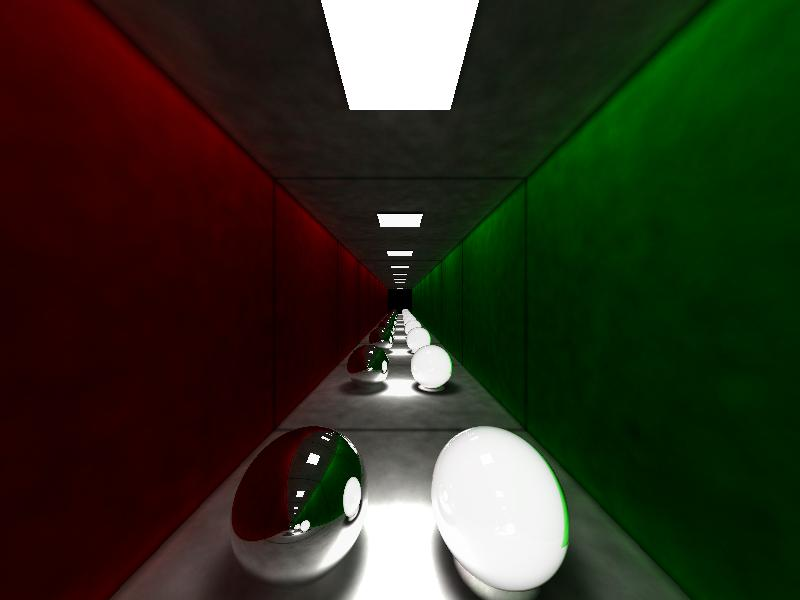
\includegraphics[width=12cm]{../outputs/two_balls_1.jpeg}
    \fcaption{Two balls (fovy=50)}\label{c1}
\end{center}

\begin{center}
    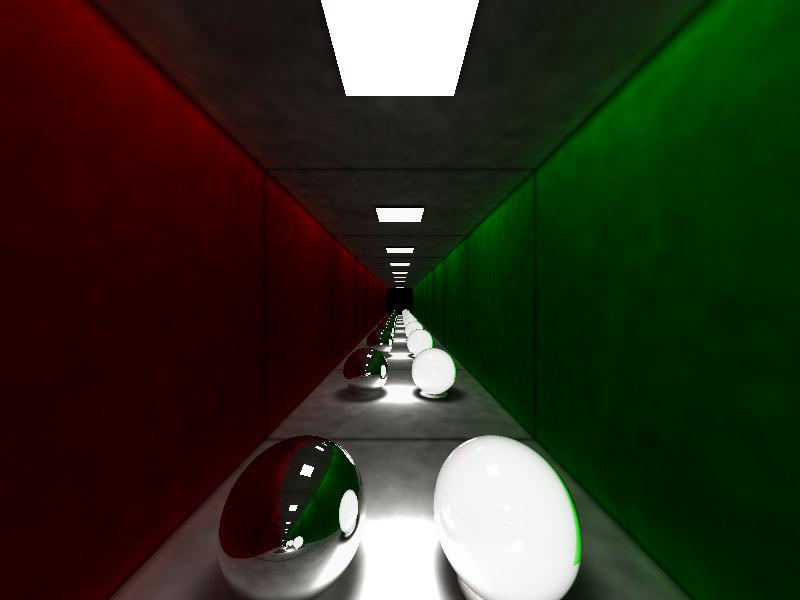
\includegraphics[width=12cm]{../outputs/two_balls_2.jpeg}
    \fcaption{Two balls (fovy=48)}\label{c2}
\end{center}

\begin{center}
    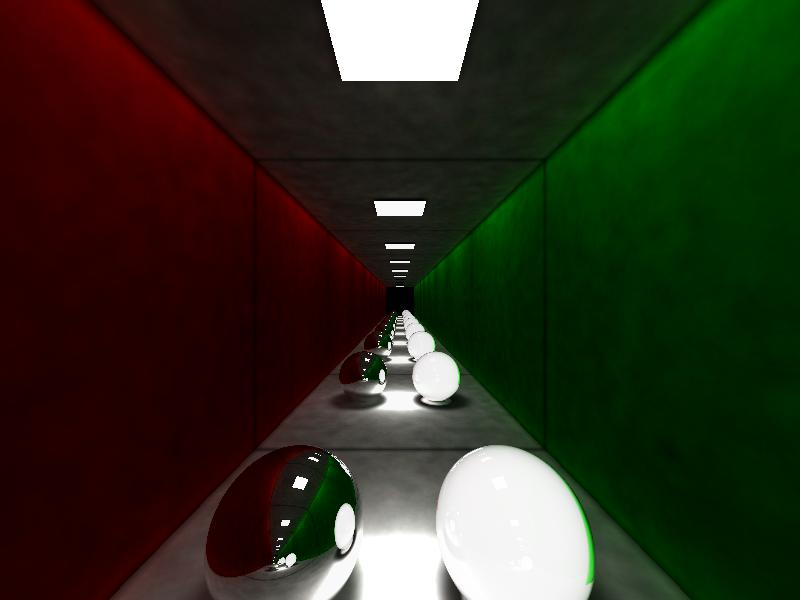
\includegraphics[width=12cm]{../outputs/two_balls_3.jpeg}
    \fcaption{Two balls (fovy=46)}\label{c3}
\end{center}

\begin{center}
    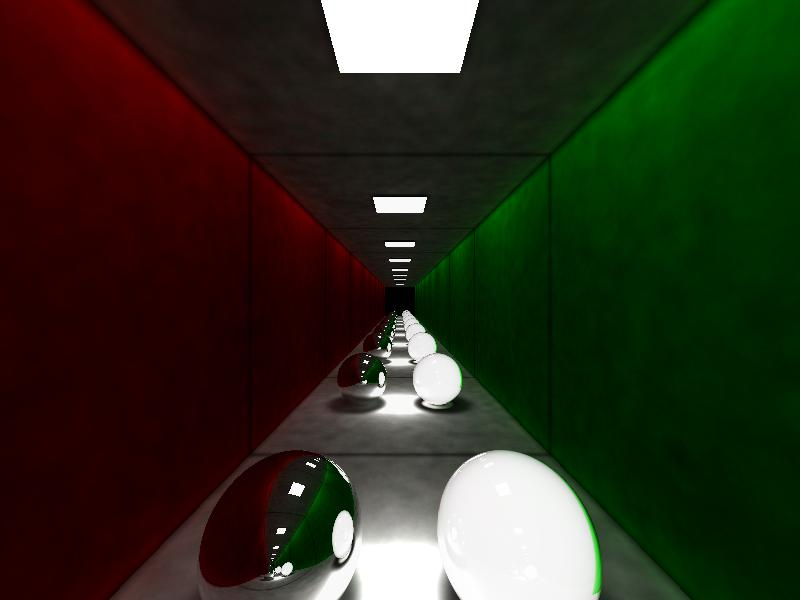
\includegraphics[width=12cm]{../outputs/two_balls_4.jpeg}
    \fcaption{Two balls (fovy=45)}\label{c4}
\end{center}

\subsection{抗锯齿}

与\fref{c4}相比,\fref{ca}进行了抗锯齿处理,图片更加清晰,这是每个像素点发射100条二维均匀分布的光线后得到的效果。

\begin{center}
    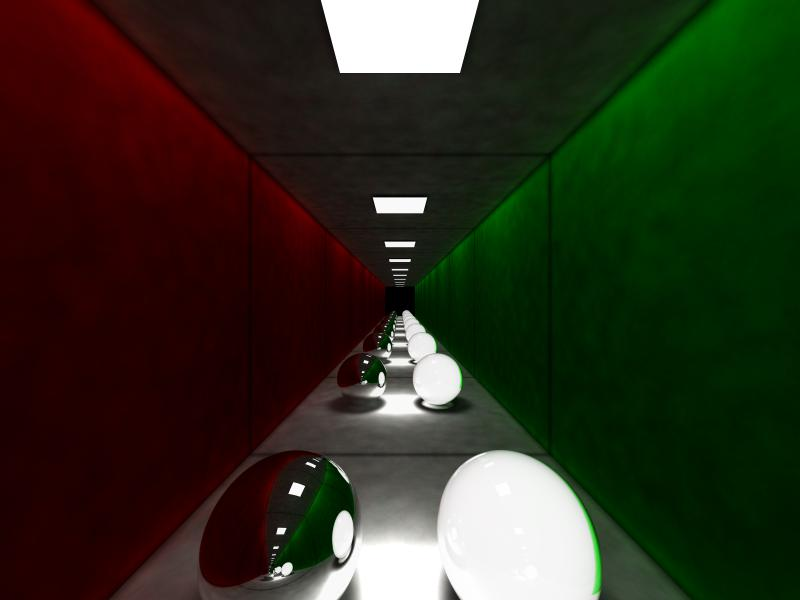
\includegraphics[width=12cm]{../outputs/anti_two_balls.jpeg}
    \fcaption{抗锯齿的Two balls}\label{ca}
\end{center}

\subsection{软阴影}

我们选取不同的曝光度 (exposure),得到\fref{e1}至\fref{e3}。可以在曝光度最大的图中清晰地看出自然的软阴影效果。

\begin{center}
    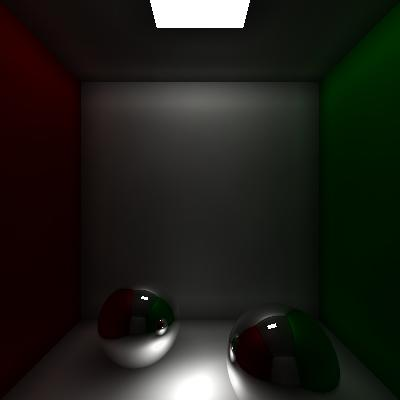
\includegraphics[width=8cm]{../outputs/balls_exp_0.01.jpeg}
    \fcaption{Balls (exposure=0.01)}\label{e1}
\end{center}

\begin{center}
    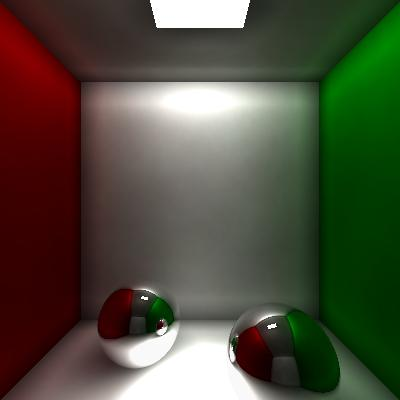
\includegraphics[width=8cm]{../outputs/balls_exp_0.03.jpeg}
    \fcaption{Balls (exposure=0.03)}\label{e2}
\end{center}

\begin{center}
    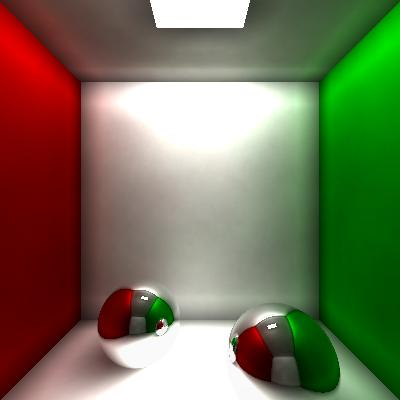
\includegraphics[width=8cm]{../outputs/balls_exp_0.05.jpeg}
    \fcaption{Balls (exposure=0.05)}\label{e3}
\end{center}

\subsection{多光源}

\fref{ml}渲染了一个具有两个呈对角线分布的面光源。

\begin{center}
    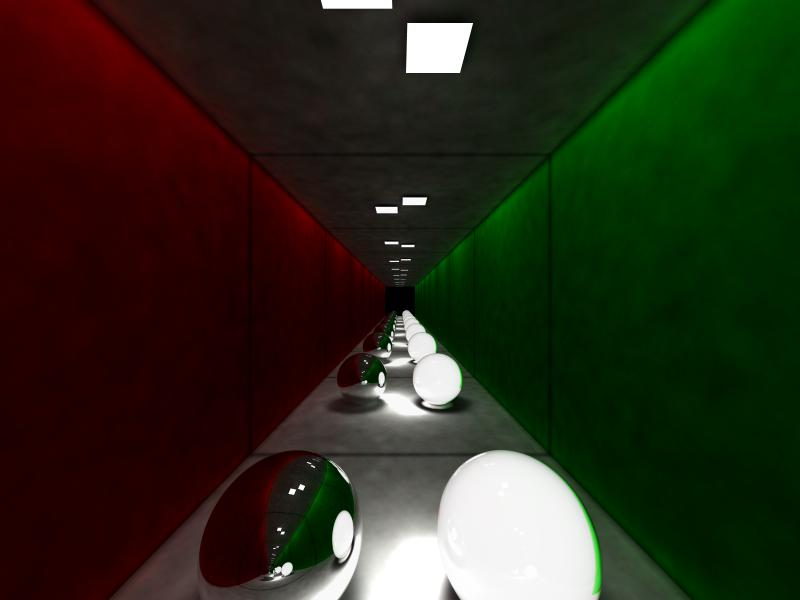
\includegraphics[width=12cm]{../outputs/anti_two_balls_multi_lights.jpeg}
    \fcaption{Two balls with multi lights}\label{ml}
\end{center}

\subsection{贴图}

\fref{tex}实现了对球面的纹理贴图。

\begin{center}
    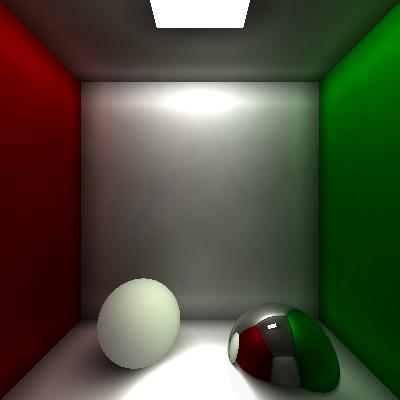
\includegraphics[width=8cm]{../outputs/texture.jpeg}
    \fcaption{简单球面贴图}\label{tex}
\end{center}

\subsection{模型渲染}

我们首先选取一个简单的模型 (\texttt{cube.obj}),对其使用普通的立方体、非加速面片渲染和KD树加速面片渲染,分别得到\fref{b1}、\fref{b2}、\fref{b3}。

\begin{center}
    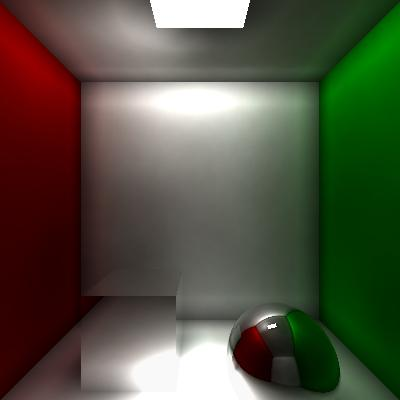
\includegraphics[width=8cm]{../outputs/box.jpeg}
    \fcaption{Box (非模型)}\label{b1}
\end{center}

\begin{center}
    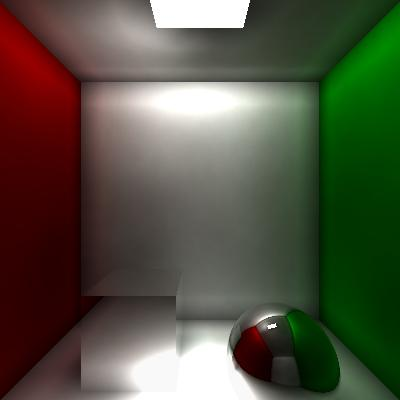
\includegraphics[width=8cm]{../outputs/box_model_slow.jpeg}
    \fcaption{Box (非加速模型)}\label{b2}
\end{center}

\begin{center}
    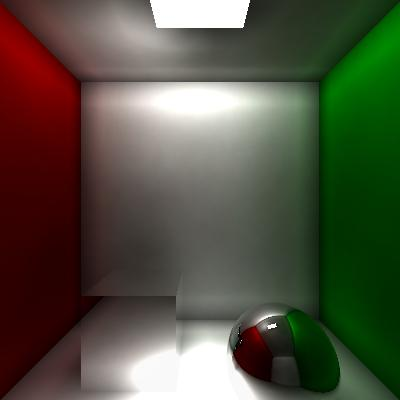
\includegraphics[width=8cm]{../outputs/box_model.jpeg}
    \fcaption{Box (加速模型)}\label{b3}
\end{center}

我们还使用一个简化了的球面模型 (\texttt{sphere.obj}) 进行非加速渲染,可以得到\label{sp}。但是使用加速渲染会出现问题,目前仍未解决。

\begin{center}
    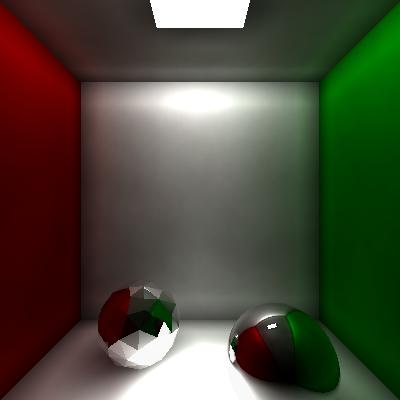
\includegraphics[width=8cm]{../outputs/sphere_model_slow.jpeg}
    \fcaption{Sphere (非加速模型)}\label{sp}
\end{center}

\section{用法}

请前往\url{https://github.com/paulzfm/PhotonMapping#photon-mapping}查看。

\begin{thebibliography}{99}
    \bibitem{1} Siggraph 2000 Course 8. A Practical Guide to Global Illumination using Photon Maps. Sunday, July 23, 2000.
    \bibitem{2} Henrik Wann Jensen. Global Illumination using Photon Maps. Department of Graphical Communication, the Technical University of Denmark.
    \bibitem{3} Tin-Tin Yu, John Lowther and Ching-Kuang Shene. Photon Mapping Made Easy. Department of Computer Science, Michigan Technological University.
    \bibitem{4} Peter Shirley, R. Keith Morley. Realistic Ray Tracing (Second Edition). A.K.Peters, Natick, Massachusetts.
    \bibitem{5} Bram de Greve. Reflections and Refractions in Ray Tracing.
\end{thebibliography}

\end{document}